\documentclass[newpage]{homework}
\newcommand{\hwname}{Zooey Nguyen}
\newcommand{\hwemail}{zooeyn@ucla.edu}
\newcommand{\hwclass}{Math 151A}
\newcommand{\hwtype}{Homework}
\newcommand{\hwnum}{5}
\begin{document}
\maketitle

\question
Piecewise linear polynomial for three points.
\begin{align*}
	f(0)	&=	0	\\
	f(0.5)	&=	0	\\
	f(1)	&=	0	\\
	P_{1,2}	&= 0
\end{align*}
Piecewise linear polynomial for five points.
\begin{align*}
	f(0)	&=	0	\\
	f(0.25)	&=	1	\\
	f(0.5)	&=	0	\\
	f(0.75)	&=	-1	\\
	f(1)	&=	0	\\
	P_{1,4}	&= \begin{cases}
		4x	&	x \in (0,0.25)	\\
		-4x+2	&	x \in (0.25,0.75)	\\
		4x-4	&	x \in (0.75,1)	\\
	\end{cases}
\end{align*}
Graph of piecewise linear interpolants.
\begin{figure}[htbp]
	\centering
	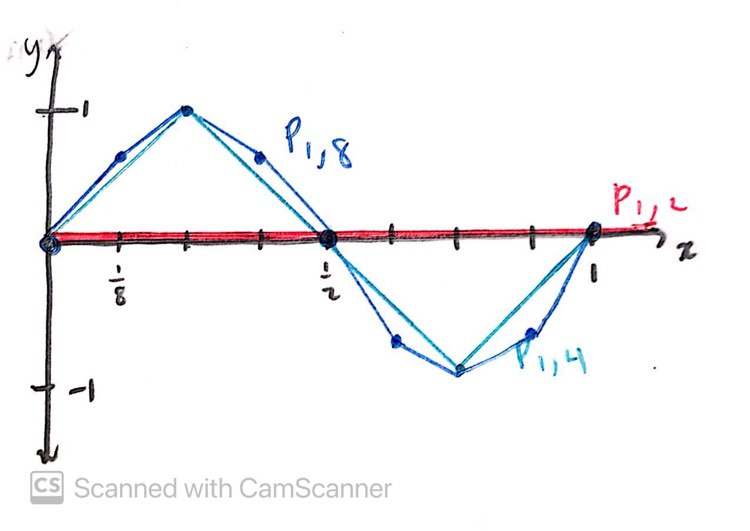
\includegraphics[width=0.5\textwidth]{1c.jpg}
\end{figure}
The pointwise error should go to 0 based on these pictures.

\question
Derivation of cubic spline.
\begin{figure}[htbp]
	\centering
	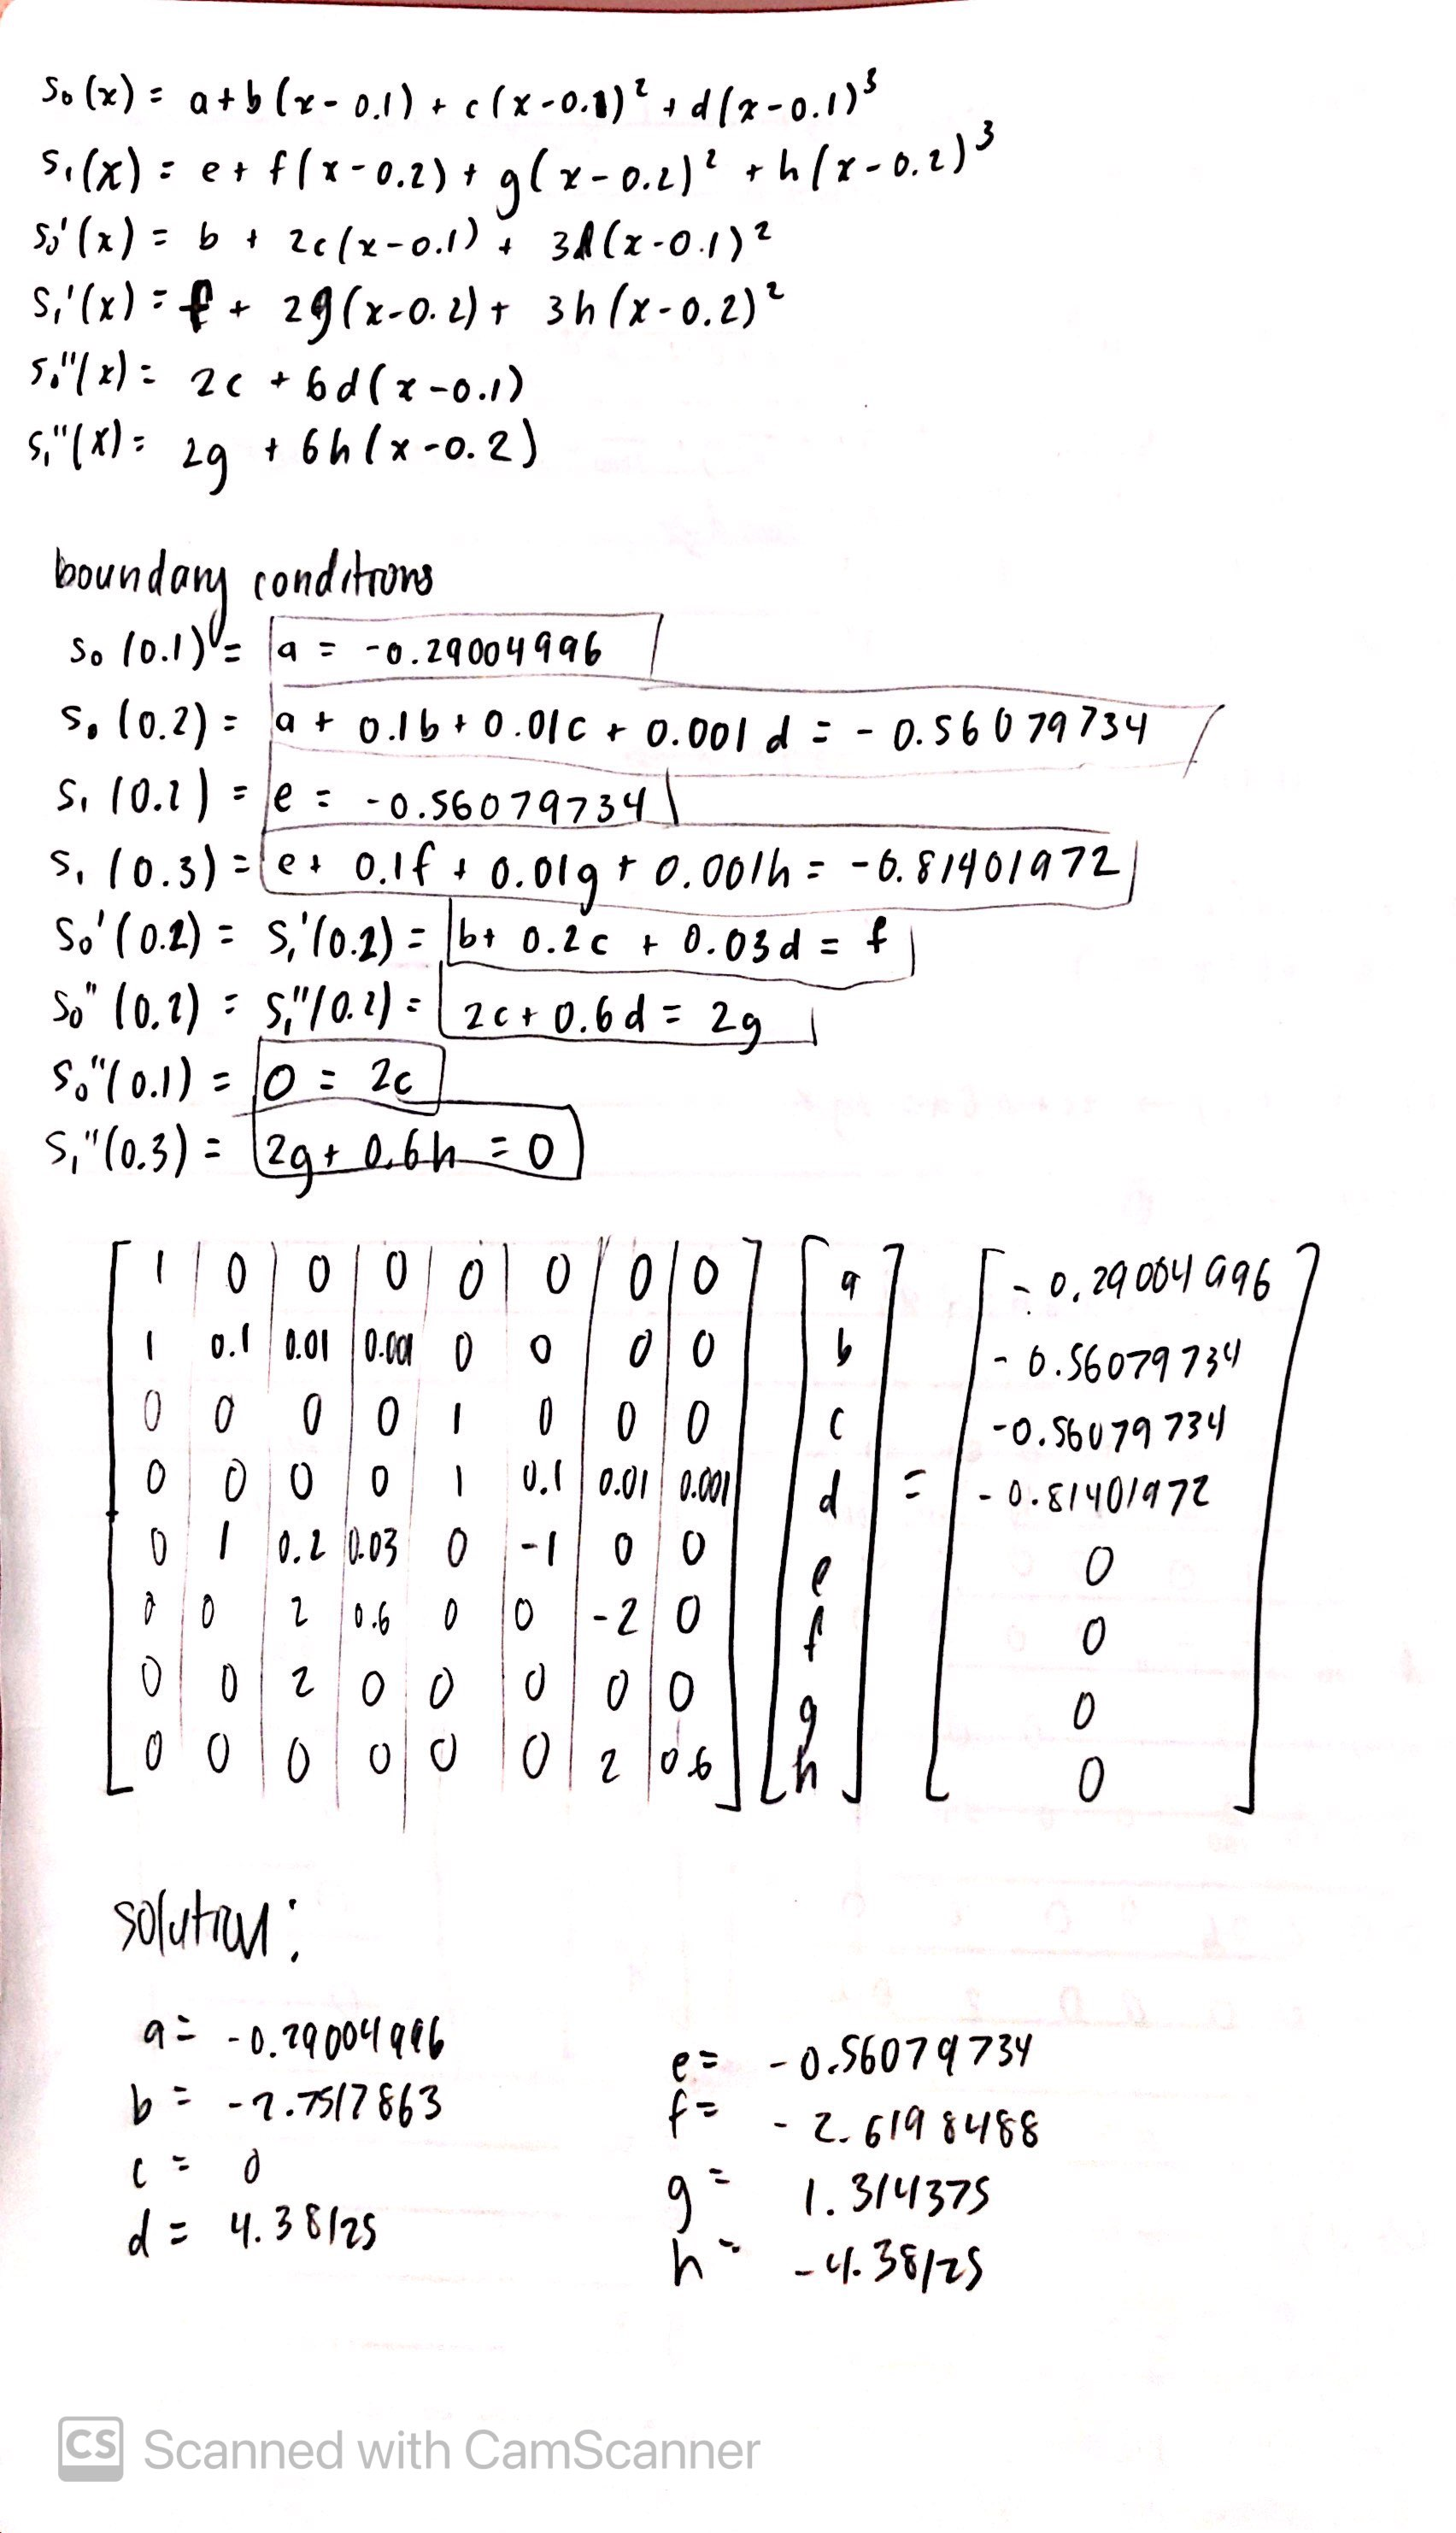
\includegraphics[width=0.4\textwidth]{3a.jpg}
\end{figure}
This gives the result:
\begin{align*}
	s(x)	&=	\begin{cases}
		-0.29004996 - 2.7512863(x-0.1) + 4.38125(x-0.1)^3	&	x \in [0.1,0.2]	\\
		-0.56079734 - 2.6198488(x-0.2) + 2.6198488(x-0.2)^2 - 4.38125(x-0.2)^3	&	x \in [0.2, 0.3]
	\end{cases}
\end{align*}
Approximations at $x=0.18$, use $s_1(x)$ since $0.18 \in [0.1, 0.2]$.
\begin{align*}
	s(0.18)	&=	-0.507909664
	&	e_{rel}	=	0.00042	\\
	s'(0.18)	&=	-2.6671575
	&	e_{rel}	=	0.00586
\end{align*}
Approximations of $f'(x)$ at $x=0.2$ comparing $s_1(x), s_2(x)$. They agree exactly. This is because in the definition of a cubic spline we required continuity of the derivative at the in-between points, or at $x=0.2$
\begin{align*}
	s_1'(0.2)	&=	13.14375(0.2)^2-2.62875(0.2)-2.619848
		=	-2.619848	\\
	s_2'(0.2)	&=	-13.14375(0.2)^2+10.4971976(0.2)-4.19353832
		=	-2.619848	\\
\end{align*}

\question
Third order Taylor expansion.
\begin{align*}
	f(x)	&=	f(x_0) + f'(x_0)(x-x_0) + \frac{f''(x_0)}{2!}(x-x_0)^2 + \frac{f^{(3)}(x_0)}{3!}(x-x_0)^3 + \frac{f^{(4)}(\xi)}{4!}(x-x_0)^4
\end{align*}
Centered difference approximation.
\begin{align*}
	f(x_0+h)	&=	f(x_0) + f'(x_0)h + \frac{f''(x_0)}{2!}h^2 + \frac{f^{(3)}(x_0)}{3!}h^3 + \frac{f^{(4)}(\xi_1)}{4!}h^4	\\
	f(x_0-h)	&=	f(x_0) - f'(x_0)h + \frac{f''(x_0)}{2!}h^2 - \frac{f^{(3)}(x_0)}{3!}h^3 + \frac{f^{(4)}(\xi_2)}{4!}h^4	\\
	f(x_0+h) + f(x_0-h)	&=	2f(x_0) + 2\frac{f''(x_0)}{2}h^2 + \frac{f^{(4)}(\xi_1) + f^{(4)}(\xi_2)}{4!}h^4	\\
	f(x_0+h) - 2f(x_0) + f(x_0-h)	&=	f''(x_0)h^2 + \frac{h^4}{4!}(f^{(4)}(\xi_1) + f^{(4)}(\xi_2))	\\
	\frac{f(x_0+h) - 2f(x_0) + f(x_0-h)}{h^2}	&=	f''(x_0) + \frac{h^2}{4!}(f^{(4)}(\xi_1) + f^{(4)}(\xi_2))	\\
\end{align*}

\question
Centered difference approximation of $f(x) = 3xe^x - \cos x$ at $x = 1.3$ with $h = 0.1, 0.01$.
\begin{align*}
	f''(1.3)	&\approx	\frac{f(1.4) - 2f(1.3) + f(1.2)}{0.01}
				=	\frac{16.86187 - 2(14.04276) + 11.59006}{0.01}
				=	36.641	\\
	f''(1.3)	&\approx	\frac{f(1.31) - 2f(1.3) + f(1.29)}{0.0001}
				=	\frac{14.30741 - 2(14.04276) + 13.78176}{0.0001}
				=	36.5	\\
	f''(1.3)	&=	3((1.3)e^(1.3)+2e^(1.3))+ \cos (1.3)
				=	36.593
\end{align*}

\end{document}
